\chapter{L'organisme~: un système en interaction avec son environnement}\label{ch:b1:organism-environment}

Un lapin est assis au bord d'une prairie, un matin de janvier. Dans
l'heure qui vient il mangera cent grammes d'herbe, respirera quelque
\qty{400}{L} d'air, perdra de la chaleur à travers son pelage vers un air
à \qty{2}{\celsius}, boira dans une flaque et détalera lorsque l'ombre
d'une buse traversera le champ. Rien de ce qu'il fait n'est possible sans
que quelque chose franchisse sa limite~: de la matière qui entre et qui
sort, de l'énergie qui entre et qui sort, de l'information qui entre. À
deux cents mètres de là, un chêne fait les mêmes choses sans bouger~: il
prélève du dioxyde de carbone et de la lumière, puise l'eau par un
système racinaire plus étendu que sa couronne, et perd cette eau dans le
même air froid. Ce chapitre énonce ce qu'est un \omterm{def:b1:organism-environment:organism}{organisme} en tant que
système, pourquoi sa taille impose sa construction, comment il maintient
son intérieur constant alors que tout change au-dehors, et comment ses
besoins énergétiques varient avec sa masse. Les deux \omterm{def:b1:organism-environment:organism}{organismes} de cette
ouverture, un mammifère et une plante à fleurs, sont les modèles auxquels
toute l'année revient.

\begin{omfigure}
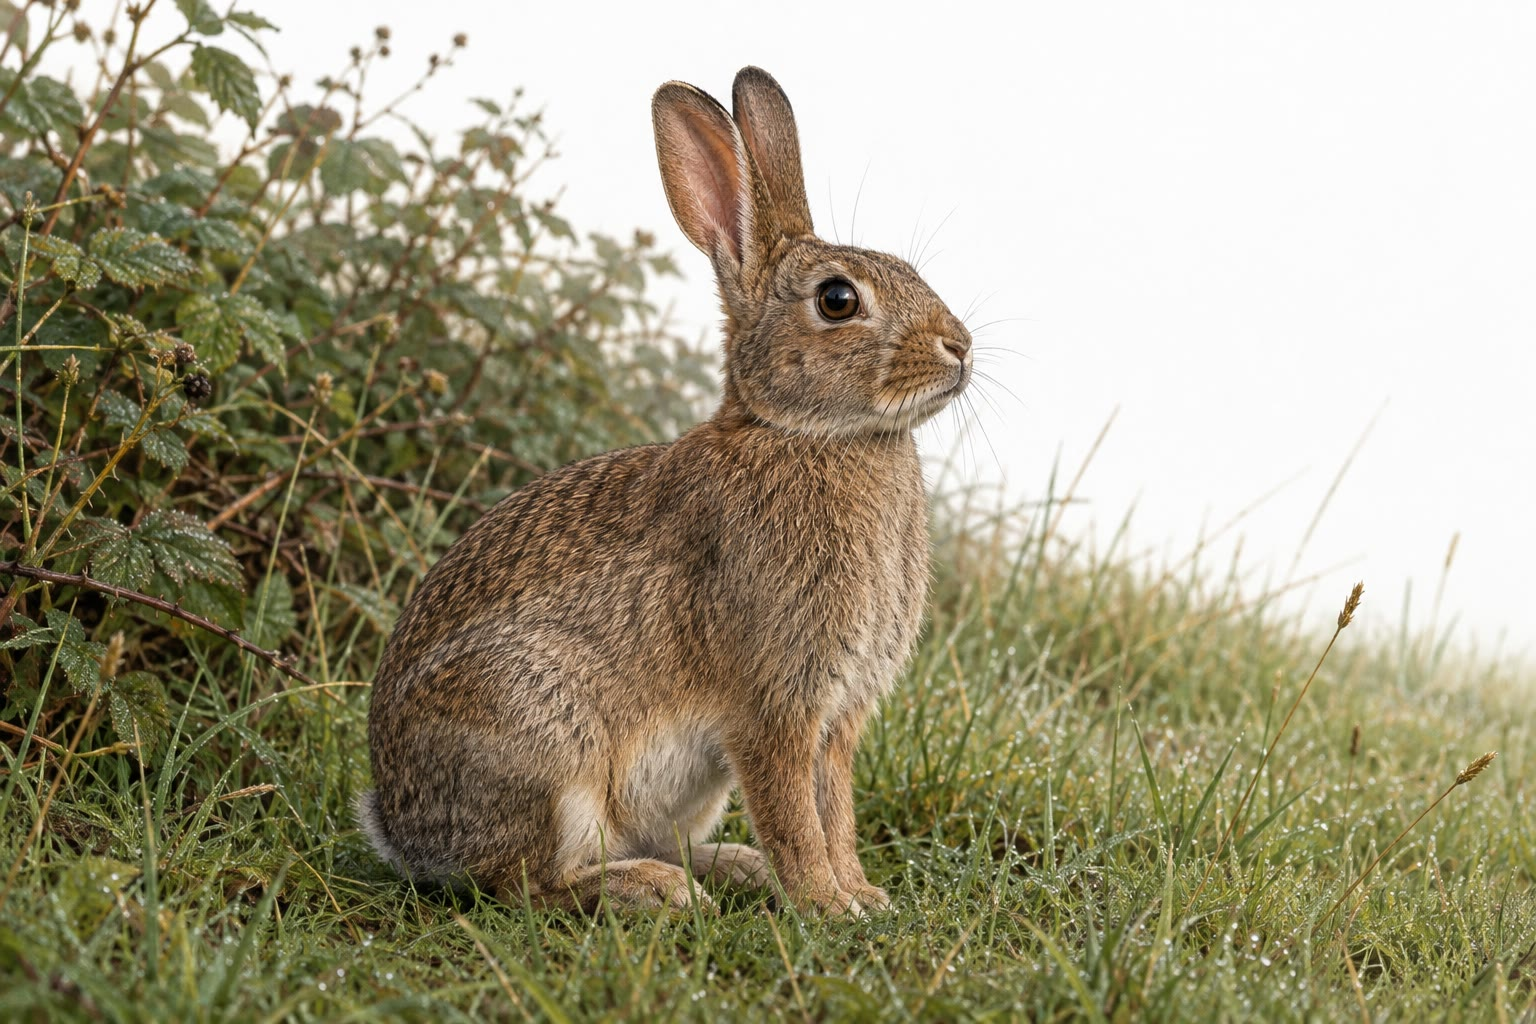
\includegraphics[width=0.62\linewidth]{images/book3/ai/b3-01-rabbit-field.jpg}

{\small Un lapin de garenne au bord d'une prairie~: en une heure il
mangera, respirera, perdra de la chaleur, boira et fuira --- chacune de
ces actions étant un échange à travers sa limite.}
\end{omfigure}

\section{Un système ouvert}

\begin{definition}[Organisme, système ouvert]\label{def:b1:organism-environment:organism}
Un \emph{organisme}\index{organisme} est un individu vivant~: un système
délimité, capable de se maintenir et de se reproduire, formé d'une
cellule ou de nombreuses cellules qui partagent une même origine et un
même fonctionnement. C'est un \emph{système ouvert}
\index{systeme ouvert@système ouvert}~: matière et énergie franchissent sa limite en
permanence, et il
ne reste vivant qu'aussi longtemps qu'elles le font.
L'\emph{environnement}\index{environnement} d'un organisme est tout ce
qui, hors de cette limite, échange avec lui --- le milieu physique (air,
eau, sol, lumière, température) et les autres organismes.
\end{definition}

\begin{proposition}[Les trois échanges]\label{prop:b1:organism-environment:exchanges}
Tout \omterm{def:b1:organism-environment:organism}{organisme} échange trois choses avec son environnement~:
\begin{itemize}
  \item de la \emph{matière}\index{echange de matiere@échange de matière}~: il prélève des
        nutriments, de l'eau et des gaz, et rejette des déchets, des gaz
        et de l'eau~;
  \item de l'\emph{énergie}\index{echange d'energie@échange d'énergie}~: il capte de
        l'énergie sous forme de lumière (\omterm{def:b1:organism-environment:trophy}{autotrophes}) ou d'énergie
        chimique des aliments (\omterm{def:b1:organism-environment:trophy}{hétérotrophes}), et la libère presque
        entièrement sous forme de chaleur~;
  \item de l'\emph{information}\index{echange d'information@échange d'information}~: il détecte
        les signaux de l'environnement (lumière, substances chimiques,
        température, contact, son) et y répond.
\end{itemize}
Sur une période pendant laquelle l'\omterm{def:b1:organism-environment:organism}{organisme} ne croît ni ne maigrit, son
bilan est fermé~: la matière entrante égale la matière sortante, et
l'énergie entrante égale la chaleur sortante augmentée du travail fourni
à l'extérieur.
\end{proposition}
\begin{proof}
Les deux premiers découlent de la conservation de la masse et de
l'énergie appliquée au volume intérieur à la limite~: ce qui s'accumule
est la différence entre l'entrée et la sortie, et un \omterm{def:b1:organism-environment:organism}{organisme} en régime
stationnaire n'accumule rien. L'énergie chimique qui n'est pas stockée
sous forme de biomasse nouvelle finit en chaleur, car chaque réaction de
l'\omterm{def:b1:organism-environment:organism}{organisme} dissipe son énergie libre en chaleur, et le travail mécanique
fourni à l'extérieur (se déplacer, soulever) est la seule autre sortie.
Le troisième est le constat qu'aucun \omterm{def:b1:organism-environment:organism}{organisme} n'est indifférent à ce qui
l'entoure.
\end{proof}

\begin{omfigure}
\begin{tikzpicture}[font=\footnotesize, >=Stealth, line cap=round]
  \draw[very thick, omDef, fill=omDef!6, rounded corners=12pt] (0,0) rectangle (4.4,3.4);
  \node[font=\small\bfseries, omDef] at (2.2,2.95) {organisme};
  \node[align=center] at (2.2,1.5) {milieu intérieur\\ cellules, tissus, organes\\ travail chimique, croissance,\\ mouvement, reproduction};
  % matter in / out
  \draw[->, thick, omProp] (-1.3,2.6) -- (0,2.6) node[pos=0, left, align=right] {nutriments, eau,\\ $\mathrm{O_2}$ ou $\mathrm{CO_2}$};
  \draw[->, thick, omProp] (4.4,2.6) -- (5.7,2.6) node[right, align=left] {déchets, eau,\\ $\mathrm{CO_2}$ ou $\mathrm{O_2}$};
  % energy
  \draw[->, thick, omThm] (-1.3,1.5) -- (0,1.5) node[pos=0, left, align=right] {énergie~: lumière, ou\\ énergie chimique des aliments};
  \draw[->, thick, omThm] (4.4,1.5) -- (5.7,1.5) node[right, align=left] {chaleur, et travail\\ fourni à l'extérieur};
  % information
  \draw[->, thick, omExo] (-1.3,0.5) -- (0,0.5) node[pos=0, left, align=right] {information~: lumière,\\ substances, température};
  \draw[->, thick, omExo] (4.4,0.5) -- (5.7,0.5) node[right, align=left] {réponses~: mouvement,\\ sécrétion, croissance};
\end{tikzpicture}

{\small L'\omterm{def:b1:organism-environment:organism}{organisme} comme \omterm{def:b1:organism-environment:organism}{système ouvert}~: matière (orange), énergie
(rouge) et information (vert) franchissent sa limite. Un \omterm{def:b1:organism-environment:organism}{organisme} en
régime stationnaire rejette autant de matière qu'il en prélève et
convertit en chaleur la quasi-totalité de l'énergie qu'il absorbe.}
\end{omfigure}

\begin{definition}[Autotrophe, hétérotrophe]\label{def:b1:organism-environment:trophy}
Un \omterm{def:b1:organism-environment:organism}{organisme} est \emph{autotrophe}\index{autotrophie} lorsqu'il
construit sa propre matière organique à partir de carbone minéral
(dioxyde de carbone) en utilisant une source d'énergie extérieure ---
la lumière pour les \emph{photoautotrophes}\index{photoautotrophe}
(plantes, algues, cyanobactéries), l'oxydation de composés minéraux pour
les \emph{chimioautotrophes}\index{chimioautotrophe}. Il est
\emph{hétérotrophe}\index{heterotrophie@hétérotrophie} lorsqu'il doit prélever de la
matière organique fabriquée par d'autres \omterm{def:b1:organism-environment:organism}{organismes}, laquelle lui
fournit à la fois son carbone et son énergie (animaux, champignons,
plupart des bactéries).
\end{definition}

\begin{example}[Le lapin et le chêne]\label{ex:b1:organism-environment:rabbitoak}
Les cent grammes d'herbe du lapin fournissent, une fois digérés, environ
\qty{500}{kJ} d'énergie chimique et le carbone de chaque molécule qu'il
construira~; l'oxygène qu'il respire lui permet d'oxyder cet aliment, et
le dioxyde de carbone qu'il expire est ce même carbone qui repart. Le
bilan du chêne est inverse~: dioxyde de carbone entrant, oxygène
sortant, l'énergie arrivant sous forme de lumière --- quelque
\qty{5}{kW} tombant sur sa couronne à midi, dont il stocke moins d'un
pour cent en sucre. Tous deux libèrent en chaleur presque toute
l'énergie qu'ils traitent~: le pelage du lapin est chaud, et les
feuilles du chêne sont refroidies par l'évaporation que leur propre
absorption de lumière entretient.
\end{example}

\section{Les échelles d'organisation et le problème de la taille}

\begin{definition}[Niveaux d'organisation]\label{def:b1:organism-environment:levels}
La matière vivante est organisée en \emph{niveaux
d'organisation}\index{niveaux d'organisation} emboîtés, chacun bâti à
partir des unités du niveau inférieur et doté de propriétés que ce
dernier n'a pas~: molécules ($\qty{1}{nm}$), cellules
($\qtyrange{1}{100}{\micro m}$), tissus, organes
($\qtyrange{1}{100}{mm}$), appareils, l'\omterm{def:b1:organism-environment:organism}{organisme} ($\qty{1}{\micro m}$ à
$\qty{100}{m}$), puis au-dessus la population, la communauté,
l'écosystème et la biosphère. Une cellule respire~; une molécule non.
Une population évolue~; un \omterm{def:b1:organism-environment:organism}{organisme} non.
\end{definition}

\begin{proposition}[Surface et volume]\label{prop:b1:organism-environment:sv}
Pour des corps de même forme et de taille caractéristique $L$, la
surface croît comme $L^2$ et le volume comme $L^3$, de sorte que le
rapport surface/volume décroît comme $1/L$~:
\[
\frac{S}{V} \propto \frac{1}{L}, \qquad
\frac{S}{V}\Big|_{\text{sphère}} = \frac{4\pi r^2}{\tfrac{4}{3}\pi r^3} = \frac{3}{r}.
\]
Tout ce qu'un \omterm{def:b1:organism-environment:organism}{organisme} échange traverse une surface, et tout ce qu'il
consomme est proportionnel à son volume~: un grand \omterm{def:b1:organism-environment:organism}{organisme} ne peut pas
nourrir son volume par sa surface externe.
\end{proposition}
\begin{proof}
Multiplier une forme par un facteur $k$ multiplie chaque aire par $k^2$
et chaque volume par $k^3$~; le rapport est multiplié par $1/k$. Pour
une sphère la formule est exacte.
\end{proof}

\begin{example}[Une bactérie et un humain]\label{ex:b1:organism-environment:svnumbers}
Une bactérie de rayon $\qty{0.5}{\micro m}$ a
$S/V = 3/r = \qty{6e6}{m^{-1}}$~: chaque micromètre cube de son
cytoplasme se trouve à moins d'un demi-micromètre de l'extérieur, et la
diffusion à travers sa membrane suffit à la nourrir entièrement. Un
humain modélisé par une sphère de \qty{70}{L} a $r = \qty{0.26}{m}$ et
$S/V = \qty{12}{m^{-1}}$, un demi-million de fois moins. La peau,
environ \qty{2}{m^2}, ne pourrait pas fournir l'oxygène que consomment
\qty{70}{kg} de tissus~; le poumon, replié dans le thorax, offre
\qty{100}{m^2}, et l'intestin, replié trois fois, \qty{30}{m^2}.
\end{example}

\begin{omfigure}
\begin{tikzpicture}
\begin{axis}[
  xbar, bar width=8pt,
  width=0.82\linewidth, height=6.2cm,
  axis x line=bottom, axis y line=left,
  xmode=log, log origin=infty, xmin=0.5, xmax=3000,
  xlabel={surface d'échange (\unit{m^2})},
  xlabel style={font=\small, at={(axis description cs:0.5,-0.13)}, anchor=north},
  symbolic y coords={peau humaine, poumon humain, intestin grêle humain, feuilles de chêne, racines de seigle, poils absorbants du seigle},
  ytick=data, tick label style={font=\small},
  enlarge y limits=0.12,
  nodes near coords, nodes near coords style={font=\scriptsize, anchor=west},
  point meta=rawx,
]
\addplot[fill=omDef!45, draw=omDef] coordinates
  {(2,peau humaine) (100,poumon humain) (30,intestin grêle humain) (300,feuilles de chêne) (240,racines de seigle) (400,poils absorbants du seigle)};
\end{axis}
\end{tikzpicture}

{\small \omterm{prop:b1:organism-environment:surfaces}{Surfaces d'échange}, en échelle logarithmique. La surface externe
d'un humain vaut \qty{2}{m^2}~; les surfaces repliées à l'intérieur, et
celles qu'une plante déploie dans l'air et dans le sol, sont dix à deux
cents fois plus grandes. (Un unique plant de seigle cultivé quatre mois
en caisse~: \qty{240}{m^2} de racines et \qty{400}{m^2} de poils
absorbants.)}
\end{omfigure}

\begin{proposition}[Les surfaces d'échange sont repliées, minces et ventilées]\label{prop:b1:organism-environment:surfaces}
Au-delà d'une taille de l'ordre du millimètre, un \omterm{def:b1:organism-environment:organism}{organisme} ne peut plus
être nourri par diffusion à travers sa surface externe. Les \omterm{def:b1:organism-environment:organism}{organismes}
pluricellulaires, quelle que soit leur taille, portent donc des
\emph{surfaces d'échange spécialisées}\index{surface d'echange@surface d'échange}, dont la
conception commune résout le même problème de quatre façons~: une grande
aire (repliement~: villosités, alvéoles, lamelles branchiales, poils
absorbants, limbes foliaires), une faible épaisseur (une couche
cellulaire ou moins entre les deux milieux), un milieu renouvelé du côté
externe (ventilation, courant d'eau, courant de transpiration), et un
système de transport du côté interne (sang, sève) qui distribue au reste
du volume ce qui a traversé la surface.
\end{proposition}
\begin{proof}
La loi de Fick (\cref{ch:b1:membranes-transport}) donne le flux à
travers une surface comme proportionnel à l'aire, à la différence de
concentration et à l'inverse de l'épaisseur~; renouveler le milieu
externe maintient une grande différence de concentration~; un système de
transport évacue ce qui a traversé et maintient basse la concentration
interne. Chacun des quatre caractères augmente le flux~; un grand
\omterm{def:b1:organism-environment:organism}{organisme} a besoin des quatre.
\end{proof}

\section{Le milieu intérieur et l'homéostasie}

\begin{definition}[Milieu intérieur]\label{def:b1:organism-environment:milieu}
Chez un animal pluricellulaire, la plupart des cellules ne sont pas en
contact avec le monde extérieur mais baignent dans un \emph{milieu
intérieur}\index{milieu interieur@milieu intérieur}~: le liquide extracellulaire (plasma
sanguin, lymphe, liquide interstitiel entre les cellules) dont
l'\omterm{def:b1:organism-environment:organism}{organisme} régule la composition, la température et le volume. Les
cellules échangent avec ce liquide~; le liquide échange avec l'extérieur
par les surfaces spécialisées. L'idée est de Claude Bernard (1865)~: la
fixité du milieu intérieur est la condition d'une vie libre et
indépendante.
\end{definition}

\begin{definition}[Homéostasie]\label{def:b1:organism-environment:homeostasis}
L'\emph{homéostasie}\index{homeostasie@homéostasie} est le maintien d'une variable
réglée du \omterm{def:b1:organism-environment:milieu}{milieu intérieur} (température, concentration en glucose, pH,
osmolarité, pression artérielle) au voisinage d'une \emph{valeur de
consigne}\index{valeur de consigne} malgré les variations extérieures.
Elle est obtenue par \emph{rétroaction négative}
\index{retroaction negative@rétroaction négative}~: un \emph{capteur} mesure la variable, un
centre intégrateur
la compare à la valeur de consigne, et un \emph{effecteur} agit dans le
sens qui annule l'écart. La variable n'est pas fixe mais oscille dans
une bande étroite autour de la valeur de consigne.
\end{definition}

\begin{omfigure}
\begin{tikzpicture}[font=\small, >=Stealth, line cap=round,
  box/.style={draw, thick, rounded corners=4pt, minimum height=9mm, minimum width=26mm, align=center, fill=white}]
  \node[box, fill=omDef!10] (var) at (0,0) {variable réglée\\ (p.~ex.\ température corporelle)};
  \node[box, fill=omProp!10] (sens) at (4.6,1.5) {capteur\\ (thermorécepteurs)};
  \node[box, fill=omThm!10] (int) at (4.6,-1.5) {centre intégrateur\\ (hypothalamus)};
  \node[box, fill=omExo!10] (eff) at (0,-3.0) {effecteurs\\ (frissons, vaisseaux, sueur)};
  \node[font=\footnotesize, align=center] (set) at (8.4,-1.5) {valeur de consigne\\ $\qty{37}{\celsius}$};
  \draw[->, thick] (var.east) -- ++(1.0,0) |- (sens.west);
  \draw[->, thick] (sens.south) -- (int.north) node[midway, right, font=\footnotesize] {valeur mesurée};
  \draw[->, thick] (set.west) -- (int.east);
  \draw[->, thick] (int.south) -- ++(0,-0.6) -| (eff.east) ;
  \draw[->, thick] (eff.north) -- (var.south) node[midway, left, font=\footnotesize, align=right] {correction,\\ opposée à l'écart};
  \draw[->, thick, gray] (-3.6,0.9) -- (var.north west) node[pos=0, above, font=\footnotesize, gray, align=center] {perturbation\\ (air froid)};
\end{tikzpicture}

{\small Une boucle de \omterm{def:b1:organism-environment:homeostasis}{rétroaction négative}. Le capteur renseigne sur la
variable, le centre la compare à la \omterm{def:b1:organism-environment:homeostasis}{valeur de consigne}, et les
effecteurs ramènent la variable. Le signe de la correction est toujours
opposé à celui de l'écart --- d'où le terme \emph{négative}.}
\end{omfigure}

\begin{proposition}[Ectothermes et endothermes]\label{prop:b1:organism-environment:thermo}
Un \emph{ectotherme}\index{ectotherme} (la plupart des invertébrés, les
poissons, les amphibiens, les reptiles) a une température corporelle qui
suit celle de son environnement~; son \omterm{def:b1:organism-environment:allometry}{intensité métabolique} croît avec
la température, en doublant à peu près tous les \qty{10}{\celsius}. Un
\emph{endotherme}\index{endotherme} (mammifères, oiseaux) maintient sa
température corporelle à une \omterm{def:b1:organism-environment:homeostasis}{valeur de consigne} en produisant de la
chaleur par son métabolisme. À l'intérieur d'une \emph{zone de
neutralité thermique}\index{zone de neutralite thermique@zone de neutralité thermique} de
températures ambiantes, il y parvient à son intensité basale, en
n'ajustant que son isolation et le débit sanguin cutané~; en dessous de
cette zone son \omterm{def:b1:organism-environment:allometry}{intensité métabolique} croît linéairement à mesure que
l'air se refroidit, car la perte de chaleur est proportionnelle à
l'écart de température et doit être compensée par la production~;
au-dessus, le refroidissement par évaporation coûte de l'eau et de
l'énergie.
\end{proposition}
\begin{proof}[Démonstration partielle]
Pour un corps à $T_b$ dans un air à $T_a$, la chaleur perdue par unité
de temps à travers sa surface vaut $P = hS\,(T_b - T_a)$ (loi de
refroidissement de Newton), où $h$ est un coefficient abaissé par le
pelage, les plumes ou la graisse. Une température stationnaire exige une
production de chaleur égale à $P$, donc linéaire en $T_a$ en dessous de
la \omterm{prop:b1:organism-environment:thermo}{zone de neutralité thermique}, de pente $-hS$. L'existence et la
largeur de la zone, où $h$ lui-même est ajusté (hérissement du pelage,
vasoconstriction cutanée), sont des faits physiologiques et non des
conséquences de l'équation.
\end{proof}

\begin{omfigure}
\begin{tikzpicture}
\begin{axis}[
  width=0.9\linewidth, height=6.4cm,
  axis x line=bottom, axis y line=left,
  xmin=-10, xmax=45, ymin=0, ymax=5.2,
  xlabel={température ambiante (\unit{\celsius})}, ylabel={intensité métabolique (en multiples du métabolisme basal)},
  xlabel style={font=\small, at={(axis description cs:0.5,-0.12)}, anchor=north},
  ylabel style={font=\small},
  tick label style={font=\small}, xtick={-10,0,10,20,30,40}, ytick={1,2,3,4,5},
  clip=false, legend style={font=\small, at={(0.97,0.97)}, anchor=north east, draw=none},
]
\addplot[very thick, omThm] coordinates {(-10,4.6) (0,3.4) (10,2.2) (20,1.0) (30,1.0) (33,1.05) (38,1.5) (42,2.2)};
\addlegendentry{endotherme (une souris)}
\addplot[very thick, omDef] coordinates {(-10,0.05) (0,0.12) (10,0.25) (20,0.5) (30,1.0) (40,2.0)};
\addlegendentry{ectotherme (un lézard)}
\draw[dashed, gray] (axis cs:20,0) -- (axis cs:20,1.0);
\draw[dashed, gray] (axis cs:30,0) -- (axis cs:30,1.0);
\node[font=\scriptsize, anchor=south, align=center] at (axis cs:25,1.15) {zone de neutralité\\ thermique};
\node[font=\scriptsize, anchor=west, align=left] at (axis cs:11,3.5) {pente $= -hS$~: la production\\ compense la perte};
\end{axis}
\end{tikzpicture}

{\small \omterm{def:b1:organism-environment:allometry}{Intensité métabolique} en fonction de la température ambiante.
Celle de l'\omterm{prop:b1:organism-environment:thermo}{endotherme} est minimale dans sa \omterm{prop:b1:organism-environment:thermo}{zone de neutralité thermique}
et croît linéairement à mesure que l'air se refroidit~; celle de
l'\omterm{prop:b1:organism-environment:thermo}{ectotherme} suit simplement la température, en doublant tous les dix
degrés.}
\end{omfigure}

\begin{example}[Une nuit à deux degrés]\label{ex:b1:organism-environment:night}
Le lapin de l'ouverture, au repos dans son terrier, produit environ
\qty{6}{W} de chaleur dans sa \omterm{prop:b1:organism-environment:thermo}{zone de neutralité thermique}. Dehors, à
\qty{2}{\celsius}, soit vingt degrés sous la limite inférieure de cette
zone, sa production doit monter à quelque \qty{12}{W}~: les frissons et
l'oxydation de ses réserves de graisse fournissent la différence, et son
temps de nourrissage s'allonge. Le lézard du même talus ne lutte pas
contre le froid~: son corps descend à \qty{3}{\celsius}, son métabolisme
tombe au vingtième de sa valeur estivale, et il ne bouge plus jusqu'au
retour du soleil.
\end{example}

\section{Intensité métabolique et masse corporelle}

\begin{definition}[Intensité métabolique, allométrie]\label{def:b1:organism-environment:allometry}
L'\emph{intensité métabolique}\index{intensite metabolique@intensité métabolique} $B$ d'un
\omterm{def:b1:organism-environment:organism}{organisme} est la vitesse à laquelle il convertit de l'énergie chimique,
mesurée en watts par sa production de chaleur ou par sa consommation
d'oxygène ($\qty{1}{L}$ d'$\mathrm{O_2}$ consommé
$\approx \qty{20}{kJ}$). Le \emph{métabolisme
basal}\index{metabolisme basal@métabolisme basal} est celui d'un \omterm{prop:b1:organism-environment:thermo}{endotherme} au repos, à
jeun, dans sa \omterm{prop:b1:organism-environment:thermo}{zone de neutralité thermique}. On dit qu'une grandeur $Y$
varie \emph{allométriquement}\index{allometrie@allométrie} avec la masse
corporelle $M$ lorsque $Y = a\,M^{b}$ avec un exposant $b \neq 1$~; en
échelles logarithmiques la relation est une droite de pente $b$.
\end{definition}

\begin{theorem}[Loi de Kleiber]\label{thm:b1:organism-environment:kleiber}
\index{loi de Kleiber}
Chez les mammifères et les oiseaux, de la musaraigne à la baleine, le
\omterm{def:b1:organism-environment:allometry}{métabolisme basal} varie comme la puissance trois quarts de la masse
corporelle~:
\[
B \approx \qty{3.4}{W}\times\left(\frac{M}{\qty{1}{kg}}\right)^{3/4}.
\]
L'intensité \emph{massique} $B/M$ décroît donc comme $M^{-1/4}$~: chaque
gramme de souris consomme de l'énergie environ vingt fois plus vite que
chaque gramme d'éléphant.
\end{theorem}
\begin{proof}[Faits expérimentaux]
Kleiber (1932) a porté la production de chaleur mesurée d'animaux de
\qty{20}{g} à \qty{600}{kg} en fonction de leur masse, en échelles
logarithmiques, et a trouvé une droite de pente $0.74$, et non le $0.67$
que prédirait une perte de chaleur proportionnelle à la surface. La
droite a depuis été prolongée sur huit ordres de grandeur en masse avec
la même pente à quelques centièmes près. Pourquoi l'exposant vaut $3/4$
plutôt que $2/3$ reste discuté~: l'explication dominante le rattache à
la géométrie des réseaux ramifiés (vaisseaux, voies aériennes) qui
délivrent l'oxygène à chaque cellule.
\end{proof}

\begin{omfigure}
\begin{tikzpicture}
\begin{loglogaxis}[
  width=0.9\linewidth, height=6.6cm,
  axis x line=bottom, axis y line=left,
  xmin=0.005, xmax=20000, ymin=0.05, ymax=6000,
  xlabel={masse corporelle (\unit{kg})}, ylabel={métabolisme basal (\unit{W})},
  xlabel style={font=\small, at={(axis description cs:0.5,-0.12)}, anchor=north},
  ylabel style={font=\small},
  tick label style={font=\small},
  xtick={0.01,0.1,1,10,100,1000,10000}, ytick={0.1,1,10,100,1000},
  log ticks with fixed point,
  clip=false,
]
\addplot[thick, omThm, domain=0.005:20000, samples=40] {3.4*x^0.75};
\addplot[only marks, mark=*, mark size=2pt, omDef] coordinates
  {(0.02,0.19) (0.3,1.3) (3,7.5) (70,80) (500,360) (4000,1700)};
\node[font=\scriptsize, anchor=west] at (axis cs:0.02,0.19) {\ souris};
\node[font=\scriptsize, anchor=west] at (axis cs:0.3,1.3) {\ rat};
\node[font=\scriptsize, anchor=west] at (axis cs:3,7.5) {\ chat};
\node[font=\scriptsize, anchor=west] at (axis cs:70,80) {\ humain};
\node[font=\scriptsize, anchor=west] at (axis cs:500,360) {\ cheval};
\node[font=\scriptsize, anchor=north] at (axis cs:4000,1300) {éléphant};
\node[font=\scriptsize, anchor=south east, omThm] at (axis cs:8000,4000) {pente $3/4$};
\end{loglogaxis}
\end{tikzpicture}

{\small La \omterm{thm:b1:organism-environment:kleiber}{loi de Kleiber}. \omterm{def:b1:organism-environment:allometry}{Métabolisme basal} en fonction de la masse
corporelle pour six mammifères, en échelles logarithmiques~: les points
s'alignent sur une droite de pente $3/4$ sur cinq ordres de grandeur de
masse.}
\end{omfigure}

\begin{method}[Lire un graphique allométrique]\label{met:b1:organism-environment:loglog}
\begin{enumerate}
  \item Porter $\log Y$ en fonction de $\log M$ (ou utiliser des
        échelles logarithmiques). Une loi de puissance $Y = aM^b$
        devient la droite $\log Y = \log a + b\log M$.
  \item L'exposant $b$ est la pente~: prendre deux points distants
        d'une décade en $M$~; $b$ est le nombre de décades dont $Y$ a
        monté. Un exposant de $1$ signifie la proportionnalité
        (isométrie)~; $b < 1$, la grandeur croît plus lentement que la
        masse~; $b > 1$, plus vite.
  \item Le préfacteur $a$ est la valeur de $Y$ en $M = 1$ (où
        $\log M = 0$).
  \item Pour comparer deux \omterm{def:b1:organism-environment:organism}{organismes}, utiliser le rapport~: $Y_2/Y_1 =
        (M_2/M_1)^b$. Par unité de masse, l'exposant devient $b-1$.
\end{enumerate}
\end{method}

\begin{example}[Souris et éléphant]\label{ex:b1:organism-environment:mouseelephant}
Une souris de \qty{20}{g}~: $B = 3.4\times 0.02^{0.75} = \qty{0.18}{W}$,
soit \qty{9}{W/kg}. Un éléphant de \qty{4}{t}~: $B = 3.4\times 4000^{0.75} =
\qty{1700}{W}$, soit \qty{0.43}{W/kg}. L'éléphant consomme dix mille
fois plus que la souris, mais chacun de ses grammes consomme vingt et
une fois moins~: $(4000/0.02)^{-1/4} = 1/21$. La souris doit manger le
dixième de sa masse chaque jour~; l'éléphant, le cinquantième. Le cœur
de la souris bat \qty{600}{} fois par minute, celui de l'éléphant
\qty{30}{}~: la fréquence cardiaque, comme $B/M$, varie en $M^{-1/4}$,
et les cœurs des deux animaux battent environ un milliard de fois dans
une vie.
\end{example}

\begin{remark}[Deux exposants d'échelle, et ce qui en découle]\label{rem:b1:organism-environment:consequences}
Beaucoup de fréquences d'un \omterm{def:b1:organism-environment:organism}{organisme} varient en $M^{-1/4}$ (fréquence
cardiaque, fréquence respiratoire, métabolisme massique) et beaucoup de
durées en $M^{+1/4}$ (longévité, gestation, âge à la maturité)~; leurs
produits, comme le nombre de battements par vie, sont alors indépendants
de la masse. Les tailles des organes varient à peu près en $M^{1}$
(cœur, poumon, volume sanguin sont une fraction fixe du corps), tandis
que les surfaces par lesquelles ils échangent varient en $M^{3/4}$ ---
ce qui explique que le poumon d'un grand animal soit plus finement
replié que celui d'un petit, et pas seulement plus gros.
\end{remark}

\section{Deux organismes modèles}

\begin{proposition}[Un mammifère et une plante à fleurs]\label{prop:b1:organism-environment:models}
Les deux \omterm{def:b1:organism-environment:organism}{organismes} pluricellulaires que cette année prend pour modèles
résolvent les problèmes ci-dessus de manières opposées. Un mammifère est
un \omterm{def:b1:organism-environment:trophy}{hétérotrophe} mobile à \omterm{def:b1:organism-environment:milieu}{milieu intérieur} régulé~: il se procure matière
et énergie en cherchant et en mangeant sa nourriture, échange par des
surfaces internes (tube digestif, poumon, rein) desservies par une
circulation, maintient constantes sa température et la composition de
son sang, et atteint une forme adulte fixée. Une plante à fleurs est un
\omterm{def:b1:organism-environment:trophy}{photoautotrophe} fixé au corps ouvert et modulaire~: elle tire énergie et
carbone de la lumière et de l'air au niveau de ses feuilles, eau et
minéraux du sol au niveau de ses racines, échange par des surfaces
externes qu'elle ne cesse d'agrandir par sa croissance tout au long de
sa vie, ne régule pas sa température, et ajuste sa forme à sa station.
Les deux chapitres suivants décrivent chacun de ces modèles.
\end{proposition}

\begin{example}[La même heure, deux bilans]\label{ex:b1:organism-environment:budgets}
Dans l'heure de l'ouverture, le lapin a converti \qty{500}{kJ} d'herbe
en chaleur, en mouvement et en un peu de croissance, tout en maintenant
son sang à \qty{39}{\celsius} et son glucose près de \qty{6}{mmol/L}~;
il l'a fait en se déplaçant vers la nourriture. Le chêne a converti
quelques centaines de kilojoules de la lumière tombée sur sa couronne en
sucre, a perdu \qty{5}{L} d'eau par ses feuilles pour cela, et a fabriqué
quelques micromètres de bois nouveau~; il l'a fait en étant là où
étaient la lumière et l'eau. Tous deux sont des \omterm{def:b1:organism-environment:organism}{systèmes ouverts}~; tous
deux se maintiennent en échangeant~; la forme de leurs échanges est la
forme de leur vie.
\end{example}

\section{Exercices}

\begin{exercise}[$\star$]\label{exo:b1:organism-environment:1}
Nommer les trois sortes d'échange entre un \omterm{def:b1:organism-environment:organism}{organisme} et son
environnement, avec un exemple de chacune pour un mammifère et un pour
une plante.
\end{exercise}

\begin{exercise}[$\star$]\label{exo:b1:organism-environment:2}
Dire ce que devient le rapport surface/volume lorsqu'une cellule
sphérique double son rayon, et pourquoi cela limite la taille des
cellules.
\end{exercise}

\begin{exercise}[$\star$]\label{exo:b1:organism-environment:3}
Définir l'\omterm{def:b1:organism-environment:homeostasis}{homéostasie} et nommer les trois composants d'une boucle de
\omterm{def:b1:organism-environment:homeostasis}{rétroaction négative}, en précisant leur identité pour la régulation de
la température corporelle.
\end{exercise}

\begin{exercise}[$\star$]\label{exo:b1:organism-environment:4}
D'après la figure des \omterm{def:b1:organism-environment:allometry}{intensités métaboliques}, de quel facteur
l'\omterm{def:b1:organism-environment:allometry}{intensité métabolique} du lézard diminue-t-elle entre
\qty{30}{\celsius} et \qty{10}{\celsius}, et de quel facteur celle de la
souris augmente-t-elle entre \qty{20}{\celsius} et \qty{0}{\celsius}~?
\end{exercise}

\begin{exercise}[$\star\star$]\label{exo:b1:organism-environment:5}
Un \omterm{def:b1:organism-environment:organism}{organisme} cubique de côté \qty{1}{mm} a besoin de \qty{1}{nmol}
d'oxygène par seconde et par millimètre cube, et sa surface peut en
absorber au plus \qty{2}{nmol/s} par millimètre carré. Peut-il vivre par
diffusion à travers sa surface~? Reprendre pour un côté de \qty{10}{mm}.
Trouver le plus grand côté qui le permette.
\end{exercise}

\begin{exercise}[$\star\star$]\label{exo:b1:organism-environment:6}
À l'aide de la \omterm{thm:b1:organism-environment:kleiber}{loi de Kleiber}, calculer le \omterm{def:b1:organism-environment:allometry}{métabolisme basal} d'un cheval
de \qty{500}{kg} et d'une musaraigne de \qty{5}{g}, ainsi que
l'intensité massique de chacun. Combien de fois sa propre masse en
nourriture, à \qty{5}{kJ/g}, la musaraigne doit-elle manger par jour si
sa dépense quotidienne vaut trois fois son \omterm{def:b1:organism-environment:allometry}{métabolisme basal}~?
\end{exercise}

\begin{exercise}[$\star\star$]\label{exo:b1:organism-environment:7}
Un humain au repos produit \qty{80}{W}. Convertir cette valeur en litres
d'oxygène consommés par minute et en kilojoules par jour. À combien de
watts correspond une ration de \qty{2000}{kcal}~?
(\qty{1}{kcal} = \qty{4.18}{kJ}.)
\end{exercise}

\begin{exercise}[$\star\star$]\label{exo:b1:organism-environment:8}
Le poumon d'un humain de \qty{70}{kg} a une \omterm{prop:b1:organism-environment:surfaces}{surface d'échange} d'environ
\qty{100}{m^2}. Si la surface pulmonaire variait comme la masse
corporelle à la puissance $3/4$, quelle serait celle du poumon d'une
souris de \qty{20}{g}, et celle d'un éléphant de \qty{4000}{kg}~?
Comparer avec la surface d'une sphère de même volume que l'animal
(masse volumique \qty{1000}{kg/m^3}).
\end{exercise}

\begin{exercise}[$\star\star$]\label{exo:b1:organism-environment:9}
Une boucle de \omterm{def:b1:organism-environment:homeostasis}{rétroaction négative} ne peut pas maintenir une variable
exactement à sa \omterm{def:b1:organism-environment:homeostasis}{valeur de consigne}. Expliquer pourquoi, à l'aide de la
boucle thermique, et dire ce qui fixe la largeur de la bande dans
laquelle la variable oscille.
\end{exercise}

\begin{exercise}[$\star\star\star$]\label{exo:b1:organism-environment:10}
Un corps perd de la chaleur au débit $P = hS(T_b - T_a)$ avec
$h = \qty{5}{W.m^{-2}.K^{-1}}$ pour un mammifère à pelage. Pour une
souris de \qty{20}{g} modélisée par une sphère de masse volumique
\qty{1000}{kg/m^3}, calculer la surface, la perte de chaleur à
$T_a = \qty{0}{\celsius}$ avec $T_b =
\qty{37}{\celsius}$, et comparer avec son \omterm{def:b1:organism-environment:allometry}{métabolisme basal} donné par la
\omterm{thm:b1:organism-environment:kleiber}{loi de Kleiber}. Que doit faire la souris~?
\end{exercise}

\begin{exercise}[$\star\star\star$]\label{exo:b1:organism-environment:11}
Si la perte de chaleur variait comme la surface ($M^{2/3}$) et la
production de chaleur suivant la \omterm{thm:b1:organism-environment:kleiber}{loi de Kleiber} ($M^{3/4}$), montrer que
les plus petits \omterm{prop:b1:organism-environment:thermo}{endothermes} sont ceux qui souffrent le plus du froid, et
qu'au-delà d'une certaine masse un animal aurait du mal à évacuer sa
chaleur. Estimer, avec $h = \qty{5}{W.m^{-2}.K^{-1}}$ et
$T_b - T_a = \qty{20}{K}$, la masse pour laquelle la production basale
égale la perte pour un corps sphérique.
\end{exercise}

\begin{exercise}[$\star\star\star$]\label{exo:b1:organism-environment:12}
«~Parce qu'une plante ne régule ni sa température ni ses liquides
internes, c'est un système plus simple qu'un animal.~» Discuter en un
paragraphe, à l'aide des deux stratégies d'échange de ce chapitre, des
surfaces que chacun utilise, et du sens de l'\omterm{def:b1:organism-environment:homeostasis}{homéostasie}.
\end{exercise}

\section{Problème~: la souris et l'éléphant}

\begin{problem}[{Problème du week-end --- deux mammifères séparés par
cinq ordres de grandeur~: leurs surfaces, leur chaleur, leur nourriture,
leur cœur et leurs années, jusqu'au rapport que prédit la loi de Kleiber}]
\label{pb:b1:organism-environment:1}
Une souris domestique a une masse de \qty{20}{g}~; un éléphant
d'Afrique, \qty{4000}{kg}. Tous deux maintiennent une température
corporelle voisine de \qty{37}{\celsius}, et tous deux sont modélisés,
lorsqu'une forme est nécessaire, par des sphères de masse volumique
\qty{1000}{kg/m^3}. La \omterm{thm:b1:organism-environment:kleiber}{loi de Kleiber} s'écrit
$B = \qty{3.4}{W}\,(M/\qty{1}{kg})^{3/4}$.

\medskip
\noindent\textbf{Partie I --- La géométrie.}
\begin{enumerate}
  \item Calculer le volume de chaque animal.
  \item Calculer le rayon de la sphère équivalente pour chacun.
  \item Calculer la surface de chaque sphère.
  \item Calculer le rapport surface/volume de chacun, et leur rapport.
  \item Montrer que ce rapport égale la racine cubique du rapport des
        masses, et le vérifier numériquement.
  \item Les souris et les éléphants réels ne sont pas des sphères. Dire,
        en le justifiant, si le rapport surface/volume réel de chacun
        est plus grand ou plus petit que celui de la sphère, et lequel
        des deux animaux s'en écarte le plus.
\end{enumerate}

\medskip
\noindent\textbf{Partie II --- La chaleur.}
La chaleur est perdue par la surface au débit $P = hS\,(T_b - T_a)$.
Prendre $h = \qty{10}{W.m^{-2}.K^{-1}}$ pour une peau nue et $T_a =
\qty{17}{\celsius}$.
\begin{enumerate}[resume]
  \item Calculer la perte de chaleur de chaque sphère nue.
  \item Calculer le \omterm{def:b1:organism-environment:allometry}{métabolisme basal} de chacun par la \omterm{thm:b1:organism-environment:kleiber}{loi de Kleiber}.
  \item Comparer perte et production pour l'éléphant. Une peau nue est-elle
        un problème pour lui~?
  \item Comparer perte et production pour la souris. Quelle valeur de $h$
        son pelage devrait-il assurer pour que la production basale
        couvre la perte~?
  \item Les oreilles d'un éléphant ajoutent \qty{4}{m^2} de surface
        mince et richement irriguée, et il les bat quand il fait chaud.
        Expliquer à quoi elles servent, à l'aide de la partie I.
  \item Expliquer pourquoi il n'existe aucun \omterm{prop:b1:organism-environment:thermo}{endotherme} de moins de
        quelques grammes, et pourquoi les plus petits (musaraignes,
        colibris) laissent leur température chuter la nuit.
\end{enumerate}

\medskip
\noindent\textbf{Partie III --- La nourriture.}
Un animal vivant en liberté dépense environ deux fois son \omterm{def:b1:organism-environment:allometry}{métabolisme
basal} sur une journée. Les graines de la souris fournissent
\qty{18}{kJ} par gramme, l'herbe fraîche de l'éléphant \qty{5}{kJ}
d'énergie digestible par gramme.
\begin{enumerate}[resume]
  \item Calculer la dépense énergétique quotidienne de chacun, en
        kilojoules.
  \item Calculer la prise alimentaire quotidienne de chacun, en grammes.
  \item Exprimer chaque prise en fraction de la masse corporelle, et
        comparer.
  \item Le tube digestif de l'éléphant mesure environ \qty{35}{m} et
        celui de la souris \qty{40}{cm}. Calculer le rapport des
        longueurs de tube digestif et le comparer au rapport des
        longueurs corporelles (les rayons de la partie I). Que suggère
        cette comparaison sur la variation d'échelle du tube digestif~?
\end{enumerate}

\medskip
\noindent\textbf{Partie IV --- Les cœurs et les années.}
La fréquence cardiaque varie comme $f = f_0\,(M/\qty{1}{kg})^{-1/4}$, la
longévité comme $\tau = \tau_0\,(M/\qty{1}{kg})^{1/4}$. Le cœur de la
souris bat \qty{600}{} fois par minute et elle vit deux ans.
\begin{enumerate}[resume]
  \item Calculer $f_0$ et $\tau_0$ à partir de la souris.
  \item Prédire la fréquence cardiaque et la longévité de l'éléphant.
  \item Calculer le nombre de battements de cœur dans la vie de chaque
        animal.
  \item Expliquer, à partir des deux exposants, pourquoi ce nombre est
        le même.
  \item Prédire la fréquence cardiaque et la longévité d'un humain de
        \qty{70}{kg} par les mêmes formules, et comparer avec les
        valeurs réelles (\qty{70}{} battements par minute, quelque
        \qty{80}{} années). Laquelle des deux prédictions échoue, et
        quelle peut en être la raison~?
  \item La fréquence respiratoire varie comme la fréquence cardiaque. La
        souris respire \qty{160}{} fois par minute~; prédire la
        fréquence respiratoire de l'éléphant, et calculer le nombre de
        battements de cœur par respiration pour chacun.
  \item Écrire l'\omterm{def:b1:organism-environment:allometry}{intensité métabolique} massique $B/M$ comme une
        puissance de $M$ et donner son exposant.
  \item Calculer $B/M$ pour la souris et pour l'éléphant.
  \item Énoncer le résultat~: le rapport de l'\omterm{def:b1:organism-environment:allometry}{intensité métabolique}
        massique de la souris à celle de l'éléphant, et la puissance du
        rapport des masses à laquelle il est égal.
\end{enumerate}
\end{problem}
